\section{Choix techniques}
Durant ce projet, nous avons copieusement abusé des mallocs. Cela pose
certains problèmes de gestion de la mémoire (principalement des \emph{memory leaks})
détectables avec \verb|valgrind|, mais cela nous avantage grandement.
En effet, cela nous permet de créer des
objets "persistents". Ils restent en mémoire jusqu'à la fin du programme
ou libération de la mémoire. Cela nous donne l'option d'utiliser des
structures de données génériques.

\subsection{Modularité}
Nous avons divisé notre projet en plusieurs modules, ce qui nous a permis d'avoir une meilleure organisation au niveau des fichiers
ainsi que dans la logique des composants. Nos structures de données ne sont utilisables qu'à l'aide d'interfaces ce qui permet de changer
l'implémention sans perturber les autres modules. 


\subsection{Structure du jeu}

\begin{minted}{c}
typedef struct {
    uint turn;
    uint max_turns;
    player_t *current_player;
    enum victory_type victory_type;
    struct world_t *world;
    array_list_t *captured_pieces_list;
    array_list_t *starting_position;
} game_t;
\end{minted}


Notre structure game\_t contient tous les éléments nécessaires pour le déroulement d'une partie du jeu.
Avec le recul et l'avancement dans le projet, une amélioration que nous voulions mettre en place mais n'avons
pas eu le temps était de remplacer les champs captured\_pieces\_list et starting\_pos par des tableaux d'array\_list.
Les tableaux seraient de taille nombre\_de\_couleurs afin d'avoir une array\_list pour chaque couleur ce qui permet
une séparation entre les pièces capturées selon leurs couleurs. Le bénéfice d'un tel changement est 
d'éviter les parcours inutiles, par exemple, lors de la libération de pièces, nous devons dans un premier temps
parcourir la liste des pièces capturées afin de récupérer seulement celles de la couleur du joueur alors
qu'avec la nouvelle implémentation cette étape n'est pas nécessaire donc il y aurait un gain de temps et
une simplification du code.  


\subsection{Implémentation des structures de données}
Premièrement toutes nos structures de données (sauf l'arbre par manque de temps)
n'exportent pas l'implémentation de la structure sous-jacente. Dans le \verb|.h|, il n'y a que la déclaration
du nom de la structure, pas son implémentation. Cela nous permet de réaliser un couplage faible
entre les différents fichiers utilisant ces structures de données.
\subsubsection{Tableau dynamique}
Pour le tableau dynamique, nous avons besoin des opérations standards 
sur une liste, à savoir l'ajout, la suppression, l'insertion, l'affectation, et la récupération.
Comme c'est un tableau sous-jacent, l'insertion et la suppression seront en complexité en temps O(n).
Il faut déplacer tous les éléments dans le tableau.
Ensuite, la récupération et l'affectation seront en complexité en temps O(1).
Enfin, l'ajout d'un élément à la fin du tableau sera en temps moyen O(log(n)).
En effet, lorsqu'on dépasse la taille du tableau, on doit allouer un nouveau tableau
pouvant contenir tous les éléments précédents et l'élément à ajouter.
L'approche naïve serait d'allouer un nouveau tableau de taille n+1. Le problème,
c'est que si on veut rajouter pas 1, mais 2 élements, on devra allouer 2 nouveaux tableaux, et donc recopier la liste complète 2 fois.
L'approche un peu plus subtile (celle qu'on a choisie), c'est de doubler la taille du tableau.
Cela évitera de devoir copier tous les éléments de la liste trop souvent. Au désavantage de gâcher un peu plus de mémoire.
\subsubsection{Arbre}
Pour notre arbre, nous avons choisi de l'implémenter avec une structure récursive.
Un noeud possède une valeur, une liste d'enfants et un parent.
Nous avons opté pour un double chaînage car nous en avions besoin pour remonter l'arbre
lors du calcul des mouvements possibles\textsuperscript{\ref{fig:example-moves}}.
Pour la liste des enfants, nous avons utilisé le tableau dynamique défini précédemment.
\subsubsection{Liste chaînée}
Nous avions aussi besoin d'une liste chaînée.
En effet, contrairement au tableau dynamique, l'affectation et la récupération sont en complexité O(n).
Mais, les opérations d'insertion et de suppression sont en O(1). En gardant
des pointeurs vers le dernier et premier élément de la liste, cela nous permet d'avoir un type
qui peut fonctionner comme une pile et une file en temps constant. Nous avions
particulièrement besoin d'une file pour le parcours en largeur\textsuperscript{\ref{alg:BFS}}.
\subsection{Structure des fichiers}

Les fichiers sont organisés en modules qui sont un couple .c et .h .  

\subsubsection{Les modules élémentaires}

Ces modules forment la base de la logique du programme.
Leurs définitions étaient imposées mais l'implémentation était libre. 

\begin{itemize}
    \item geometry : Gère les types de base ainsi que les définitions du projet.
    \item world : Gère les interactions avec le monde du jeu tel que placer ou récupèrer des pièces.
    \item neighbors : Gère les fonctionnalités pour récupèrer les voisins d'une case.
\end{itemize}

Les modules \emph{world} et \emph{neighbors} dépendent de \emph{geometry}.


\subsubsection{Le module util}
\label{ssec:module-util}
Nous avons décidé d'utiliser un module \emph{util} dont la majorité des autres modules inclut. 
Ce module contient les interfaces système comme \emph{stdio.h}, des définitions comme \emph{limit.h},
des définitions de type que nous utilisons dans l'ensemble du code tel que \emph{uint} pour représenter
le type \emph{unsigned int} ou des structures ainsi que des fonctions d'erreur. Nous n'avons pas eu le temps
mais les fonctions d'erreur auraient pu avoir leur propre module \emph{erreur} afin d'avoir une meilleur organisation.

Notre choix de l'utilisation de ce module est de pouvoir enrichir les fichiers élémentaire que nous ne pouvions pas 
modifier ainsi que d'avoir à seulement inclure un fichier en en-tête des autres.  


\subsubsection{Les modules}

\begin{itemize}
    \item Le module distance permet d'avoir la distance de chaque cases vers une position gagnante.
    Cela nous permet de calculer les meilleurs mouvements pour une pièce.
    Son implémentation est détaillée dans la section \ref{distance}. 
    
    \begin{figure}[H]
        \centering 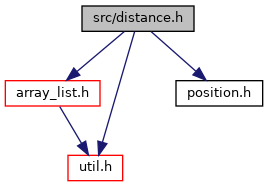
\includegraphics[width=5cm]{images/distance_8h__incl.png}
        \caption{Dépendances du module distance}
        \label{fig:dep-distance}
    \end{figure}

    \item  Le module \emph{configuration} permet de répondre à l'achievement 5, il encapsule toutes les fonctions
    liées aux paramétrages des configurations. 
    \begin{figure}[H]
        \centering 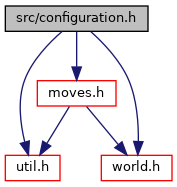
\includegraphics[width=5cm]{images/configuration_8h__incl.png}
        \caption{Dépendances du module configuration}
        \label{fig:dep-config}
    \end{figure}

    \item Le module moves contient la logique qui permet de récupèrer les mouvements possible pour
    les différents type de pièces. Toute l'implémentation est cachée dans le .c exposant seulement une fonction
    \emph{get\_moves} ce qui simplifie l'usage.
    \begin{figure}[H]
        \centering 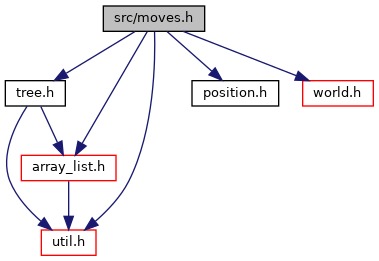
\includegraphics[width=5cm]{images/moves_8h__incl.png}
        \caption{Dépendances du module moves}
        \label{fig:dep-moves}
    \end{figure}

    \item Input est un petit module qui gère les entrées utilisateur sur le terminal. Il ne dépend de rien.

    \item Player sert à la gestion des joueurs dans le jeu. Sa seule dépendance est le module util.

    \item Le module player\_handler permet l'intéractivité entre le jeu et un ou plusieur joueurs humains via le terminal.
    \begin{figure}[H]
        \centering 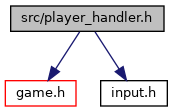
\includegraphics[width=5cm]{images/player__handler_8h__incl.png}
        \caption{Dépendances du module player\_handler}
        \label{fig:dep-playerhandler}
    \end{figure}

    \item Enfin le module game s'occupe de l'éxécution d'une partie du jeu. 
    \begin{figure}[H]
        \centering 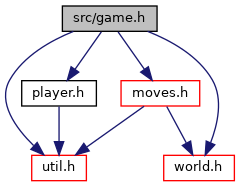
\includegraphics[width=5cm]{images/game_8h__incl.png}
        \caption{Dépendances du module game}
        \label{fig:dep-game}
    \end{figure}

\end{itemize}



Tous ces modules sont inclus dans le fichier de plus haut niveau \emph{projet} qui s'occupe 
d'initialiser le jeu puis de lancer la partie.
Le graphique complet de dépendance
de celui-ci est disponible en annexe, figure \ref{fig:dep-projet}. Avec ce graphique on peut voir l'entièreté des dépendances depuis \emph{projet}. 






